\chapter{O teto do que se aprende}\label{cap:teto}

O capítulo da tolerância contou duas explicações de cento e oitenta, e o número ficou impresso como
se fosse uma propriedade do dado. Ele não é: é o \textbf{máximo} de uma família, e um máximo depende de
duas coisas que ninguém declarou --- quantas peças foram tentadas e quantos dias foram vistos. Este
capítulo varia as duas.

\section{A contagem é um máximo}

A peça que cabe é a que passa nas quatro tolerâncias ao mesmo tempo, e o que se conta é quantas
passam. Isso é um máximo sobre as tentativas: quanto mais peças se experimenta, mais fácil é que
alguma passe por acaso. E quanto mais dias se vê, mais difícil fica.

A conta do acaso é simples o bastante para ser dita. Se cada peça passa nas quatro provas com
chance $p$, independente das outras, então:

\begin{proposicao}[o teto das tentativas]\label{prop:teto-tentativas}
A chance de que ao menos uma peça da família passe é $1-(1-p)^{m}$, que cresce com o número de
peças tentadas $m$ e tende a um. E o número esperado de peças que passam é $mp$, de modo que
\textbf{a contagem mede $m$ e $p$ juntos}, e não o que o dado sabe.
\end{proposicao}

\begin{proof}
As $m$ peças são independentes com a mesma chance $p$ de passar, de modo que a chance de nenhuma
passar é $(1-p)^{m}$ --- e o complemento é o que a proposição afirma. O número esperado de sucessos
é $mp$ pela linearidade da esperança, que não precisa de independência. Como $1-(1-p)^{m}$ cresce em
$m$ para todo $p$ no intervalo, o teto sobe com o número de tentativas.
\end{proof}

A proposição não diz que as peças são de fato independentes --- não são, e o capítulo da bateria já
mediu o quanto isso pesa. Ela diz o que a contagem carrega: um fator $m$ que o leitor não vê.

\section{Medindo as duas coisas}

A família do capítulo da tolerância tem \numTetoPecasMaior{} peças na grade cheia e
\numTetoPecasMenor{} na grade mais grossa, e a série tem seis mil setecentos e dezoito dias. Variando
as duas coisas separadamente --- a grade por um lado, o comprimento da série por outro ---, a
contagem sai assim.

\begin{table}[htbp]
  \centering
  \small
  \begin{tabular}{lrrr}
    \hline
    peças tentadas & \numTetoDiasMenor{} dias & \numTetoDiasMeio{} dias & \numTetoDiasMaior{} dias \\
    \hline
    
    \numTetoPecasMenor & \numTetoDoisQuinhentos & \numTetoDoisDoisMil & \numTetoDoisSeisMilSetecentosEDezoito \\
    
umTetoPecasMaior & \numTetoSeisQuinhentos & \numTetoSeisDoisMil & \numTetoSeisSeisMilSetecentosEDezoito \\
    \hline
  \end{tabular}
  \caption{As explicações que cabem na mesma tolerância, contra o tamanho da família e o número de
    dias vistos. A série é a do primeiro mercado, truncada.}
  \label{tab:teto}
\end{table}

Nas duas direções o número se move, e é isso que o capítulo da tolerância não dizia. Com a série
inteira e a grade cheia, cabem as duas de sempre. Com quinhentos dias e a mesma grade cheia, cabem
\numTetoSeisQuinhentos{} --- quase dez vezes mais, e nenhuma peça nova foi inventada: o que mudou
foi quanto se viu. E com a grade grossa e quinhentos dias, cabem \numTetoDoisQuinhentos{} das \numTetoPecasMenor{} peças --- uma em cada oito,
num dado que tem quinhentos dias.

\begin{figure}[htbp]
  \centering
  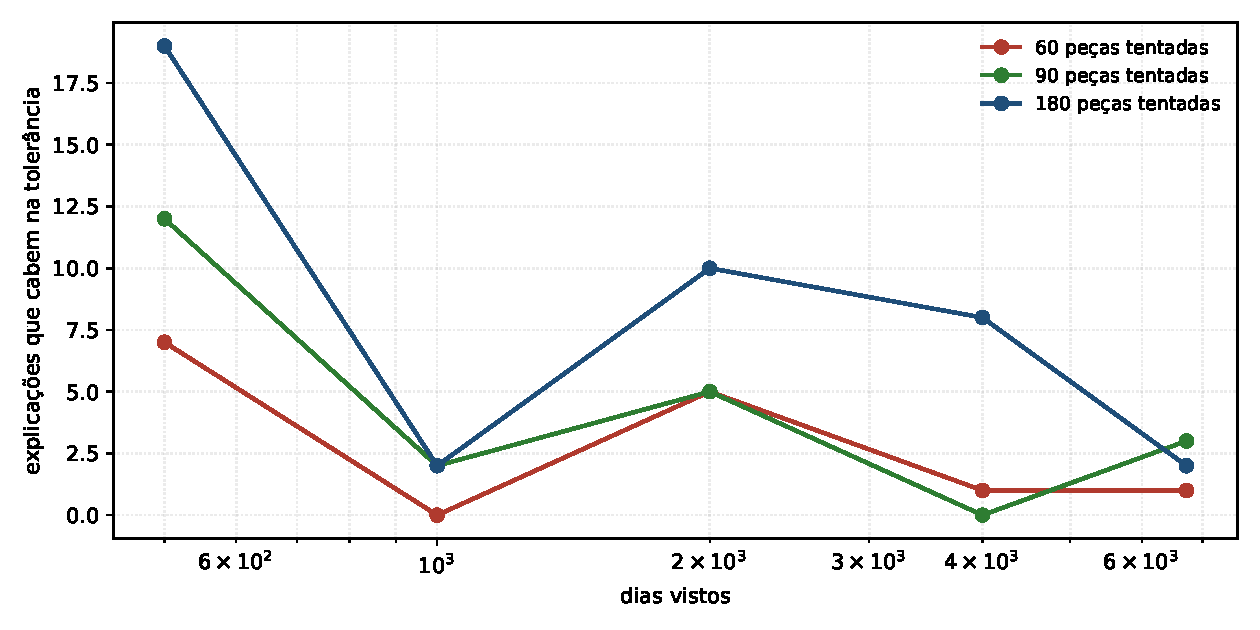
\includegraphics[width=\linewidth]{figuras/E28_teto_1.pdf}
  \caption{As explicações que cabem, contra os dias vistos, uma curva por tamanho de família. O eixo
    dos dias é logarítmico. As curvas descem conforme o dado cresce: o mesmo critério, com mais
    dias, admite menos.}
  \label{fig:teto}
\end{figure}

\section{O que fica}

Fica uma correção de leitura, e ela vale para todo o livro. \textbf{A contagem de explicações que
cabem não mede o que o dado sabe}: ela mede quantas peças foram tentadas e quantos dias foram
vistos. O número do capítulo da tolerância --- duas de cento e oitenta --- é um ponto de uma
superfície, e o ponto é honesto só quando as duas coordenadas são declaradas junto dele.

O que sobra é o fracasso seguinte, e é o que este capítulo deixa de pé. Escolher entre as
explicações que passam não é escolher entre iguais: é escolher \textbf{depois de ter olhado o dado}, e
quem escolhe assim já gastou parte da evidência que tinha. Quanto custa essa escolha é a pergunta
que o enquadramento vai medir --- depois de medir as três bordas que ele declara.
